\documentclass[main.tex]{subfiles}
\begin{document}

\section{Briefly describe \textit{Controller Area Network} (CAN)?}

\spoilerline
\noindent \textit{Controller Area Network} (CAN) is a popular communication protocol developed by Bosch in the 1980's \cite{cadence_canbus_history}. It's widely used in the automotive and robotics industries due to its robustness, reliability, and tailor-made features for automotive-type environments.\newline
\newnoindentpara \textit{Note that CAN is a fairly complex protocol, and depending on the interviewee's knowledge level about the protocol, can cause an answer to this question to get quite deep and involved. However, this answer describes some of the primary features of CAN that are integral to its operation, as many of those features are asked as standalone questions or elaborated upon in an interview setting.} \newline

\subsection{CAN Physical Layer}
The CAN standard defines the physical and data link layers of the OSI model. The physical layer uses a \textbf{differential pair} of wires (\textit{CAN\_H and CAN\_L}) to transmit data, as opposed to a single wire. It is an open-drain bus, meaning that the bus is pulled to a dominant state (logical 0) by a node asserting a dominant state (pulling \texttt{CAN\_H} to 2V above \texttt{CAN\_L}), while a recessive state (logical 1) is achieved by no node asserting a dominant state (\texttt{CAN\_H} and \texttt{CAN\_L} at the same potential) - this is shown in figure \ref{fig:can-dominant-recessive}. Note that CAN requires a transceiver to output the differential signal. Commonly microcontrollers with a CAN peripheral communicates over serial with two single ended signals, \textit{CAN\_TX} and \textit{CAN\_RX}, to a transceiver IC (\textit{Integrated Circuit}) which drives and receives the differential signals on the CAN bus. 
% Not mentioning voltages relative to ground for each signal is deliberate to avoid confusion with permissibility of common-mode offsets which is elaborated on in a subsequent paragraph. See issue #71 in Github.

\begin{figure}[H]
    \centering
    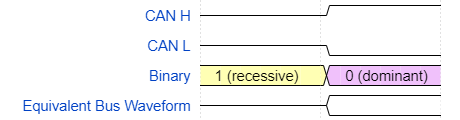
\includegraphics[width=0.6\textwidth]{generated_images/svg_generated/can_dominant_recessive.png}
    \caption{Recessive and dominant bits waveform \cite{ti_can_signal_levels}}
    \label{fig:can-dominant-recessive}
\end{figure}

\subsubsection{Differential Pair} 
A differential pair works by creating two signals: a positive signal, and a negative signal (which is the logical inverse of the positive signal). Both signals are transmitted simultaneously to the receiver, which can then subtract the two signals to recover the original data. A schematic implementation of a differential receiver is shown in figure \ref{fig:diff-physical-layer}, with a sample digital message shown in figure \ref{fig:diff-digital-sample}. \footnote{In the case of CAN, the dominant state (0) is when the CAN\_H signal is higher than the CAN\_L signal, and the recessive state is when the CAN\_H and CAN\_L signals are at the same voltage level. However, differential signals are often implemented with a different convention, where a logical 1 is signaled when $V_{positive}  > V_{negative}$, and a logical 0 is signaled when $V_{negative} > V_{positive}$}.
\begin{figure}[H]
    \centering
    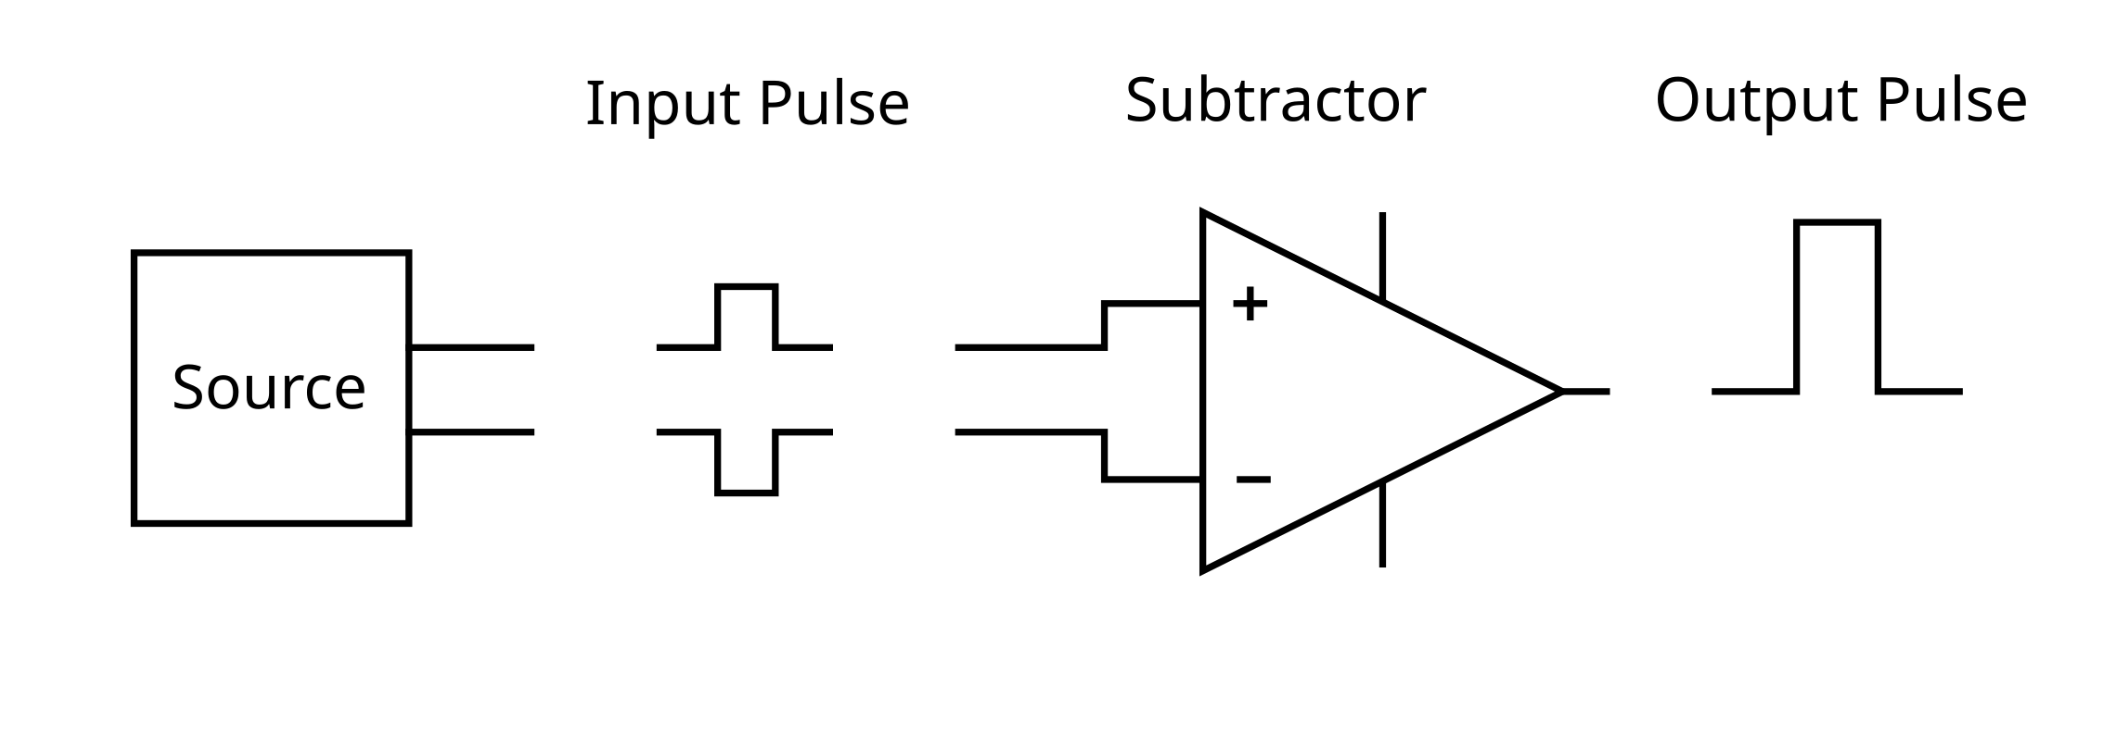
\includegraphics[width=0.6\textwidth]{images/wikipedia_diff_signal.png}
    \caption{Differential Pair Physical Layer, Source: Wikipedia \cite{wikipedia_differential_signalling}}
    \label{fig:diff-physical-layer}
\end{figure}
\begin{figure}[H]
    \centering
    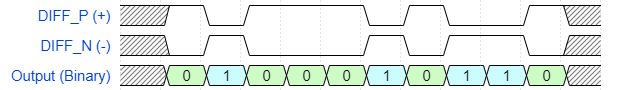
\includegraphics[width=0.75\textwidth]{generated_images/svg_generated/diff_digital_signal.png}
    \caption{Digital Differential Signal Sample}
    \label{fig:diff-digital-sample}
\end{figure}

\noindent An advantage of using a differential pair is that it reduces the impact of EMI (\textit{Electromagnetic Interference}) on the signal, as any interference will affect both wires equally. This allows the receiver to subtract the two signals, effectively removing the interference. The schematic in figure \ref{fig:diff-physical-layer-noise} shows how the receiver can subtract the two signals to remove noise.

\begin{figure}[H]
    \centering
    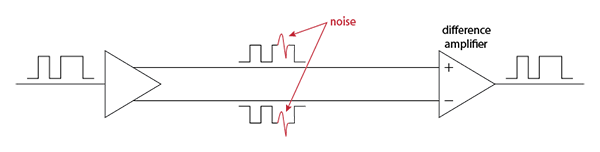
\includegraphics[width=0.8\textwidth]{images/diff_pair_noise_immunity.png}
    \caption{Differential Pair Physical Layer with Noise, Source: Stack Overflow \cite{stackoverflow_diff_pair_noise}}
    \label{fig:diff-physical-layer-noise}
\end{figure}

\noindent Another advantage of this configuration is immunity to common mode voltage offsets. Ideally, CAN transceivers are designed to output a dominant state with \texttt{CAN\_H} at 3.5V and \texttt{CAN\_L} at 1.5V, and a recessive state with \texttt{CAN\_H} and \texttt{CAN\_L} both at 2.5V. However, an advantage of differential signalling is that these values can be offset (referred to as \textit{voltage shifting}) if two transceivers have a voltage potential difference between their ground planes. More accurately, we can define a dominant state as \texttt{CAN\_H} at \(3.5 + N\)~V and \texttt{CAN\_L} at \(1.5 + N\)~V, and a recessive state as \texttt{CAN\_H} and \texttt{CAN\_L} both at \(2.5 + N\)~V. Note that there is a limit to how large \(N\) can be, depending on the specific CAN transceivers being used.

\noindent Voltage shifts in ground potential are common in embedded systems with high current power transmission; consider a motor controller may be interfaced with CAN and be receiving power from a controller board. Due to the high current going to the motor and the parasitic resistance of the wire, a potential difference due to Ohm's Law arises between the ground on the controller and the ground on the motor controller. CAN is very robust to this small change in potential whereas a single ended signal could suffer logic level issues. \newline
% @sahil Do you think this requires more of an explanation and/or any drawings to make this clear?

\noindent CAN wires are often twisted as the current flow in the signal lines is in opposing directions. When the differential pair wires are twisted, the magnetic field created by current flow in opposing directions for each bus state change in adjacent half-twists are in opposite directions and cancel each other out. Twisting wires also allows some control over the characteristic impedance. Note that CAN is very forgiving and outside of production applications and more complex bus topologies, twisting CAN wires is unnecessary for successful data transmission. 

\subsection{Bus Topology}
CAN uses a \textbf{multi-master} communication scheme, meaning that any node on the bus can initiate a message transmission. This is in contrast to a \textbf{master-slave} communication scheme, where only the master can initiate communication. They are connected in a \textbf{bus topology}, where all nodes are electrically \footnote{Physically, they may be connected differently, however, this answer only focuses on the electrical connection} connected in parallel. Essentially, every node on the bus can see every message transmitted on the bus, and every node has the ability to initiate message transmission. Note that the CAN bus is \textit{asynchronous}, meaning every node must know the bus \textit{bitrate} beforehand to understand transmissions from other nodes.
\newline
\newnoindentpara
The bus is terminated with ~120 ohm resistance at both ends to prevent signal reflections in the transmission line and to ensure that a recessive bus state can be caused when no device is asserting a dominant state. A schematic of a simple bus topology is shown in figure \ref{fig:bus-topology} with a termination at each end of the bus and a small branch length. Buses may feature more complex topologies necessitating more terminations due to different branches in the bus. CAN is a very resilient protocol, especially for lower data-rates so optimizing electrically is often unnecessary for simple small busses as long as at least one termination is present. For production applications guidelines for bus topologies, terminations, and termination values are given in standards, but are often optimized by testing from EMC (\textit{Electro-Magnetic Compliance}) engineers in the lab.

\begin{figure}[H]
    \centering
    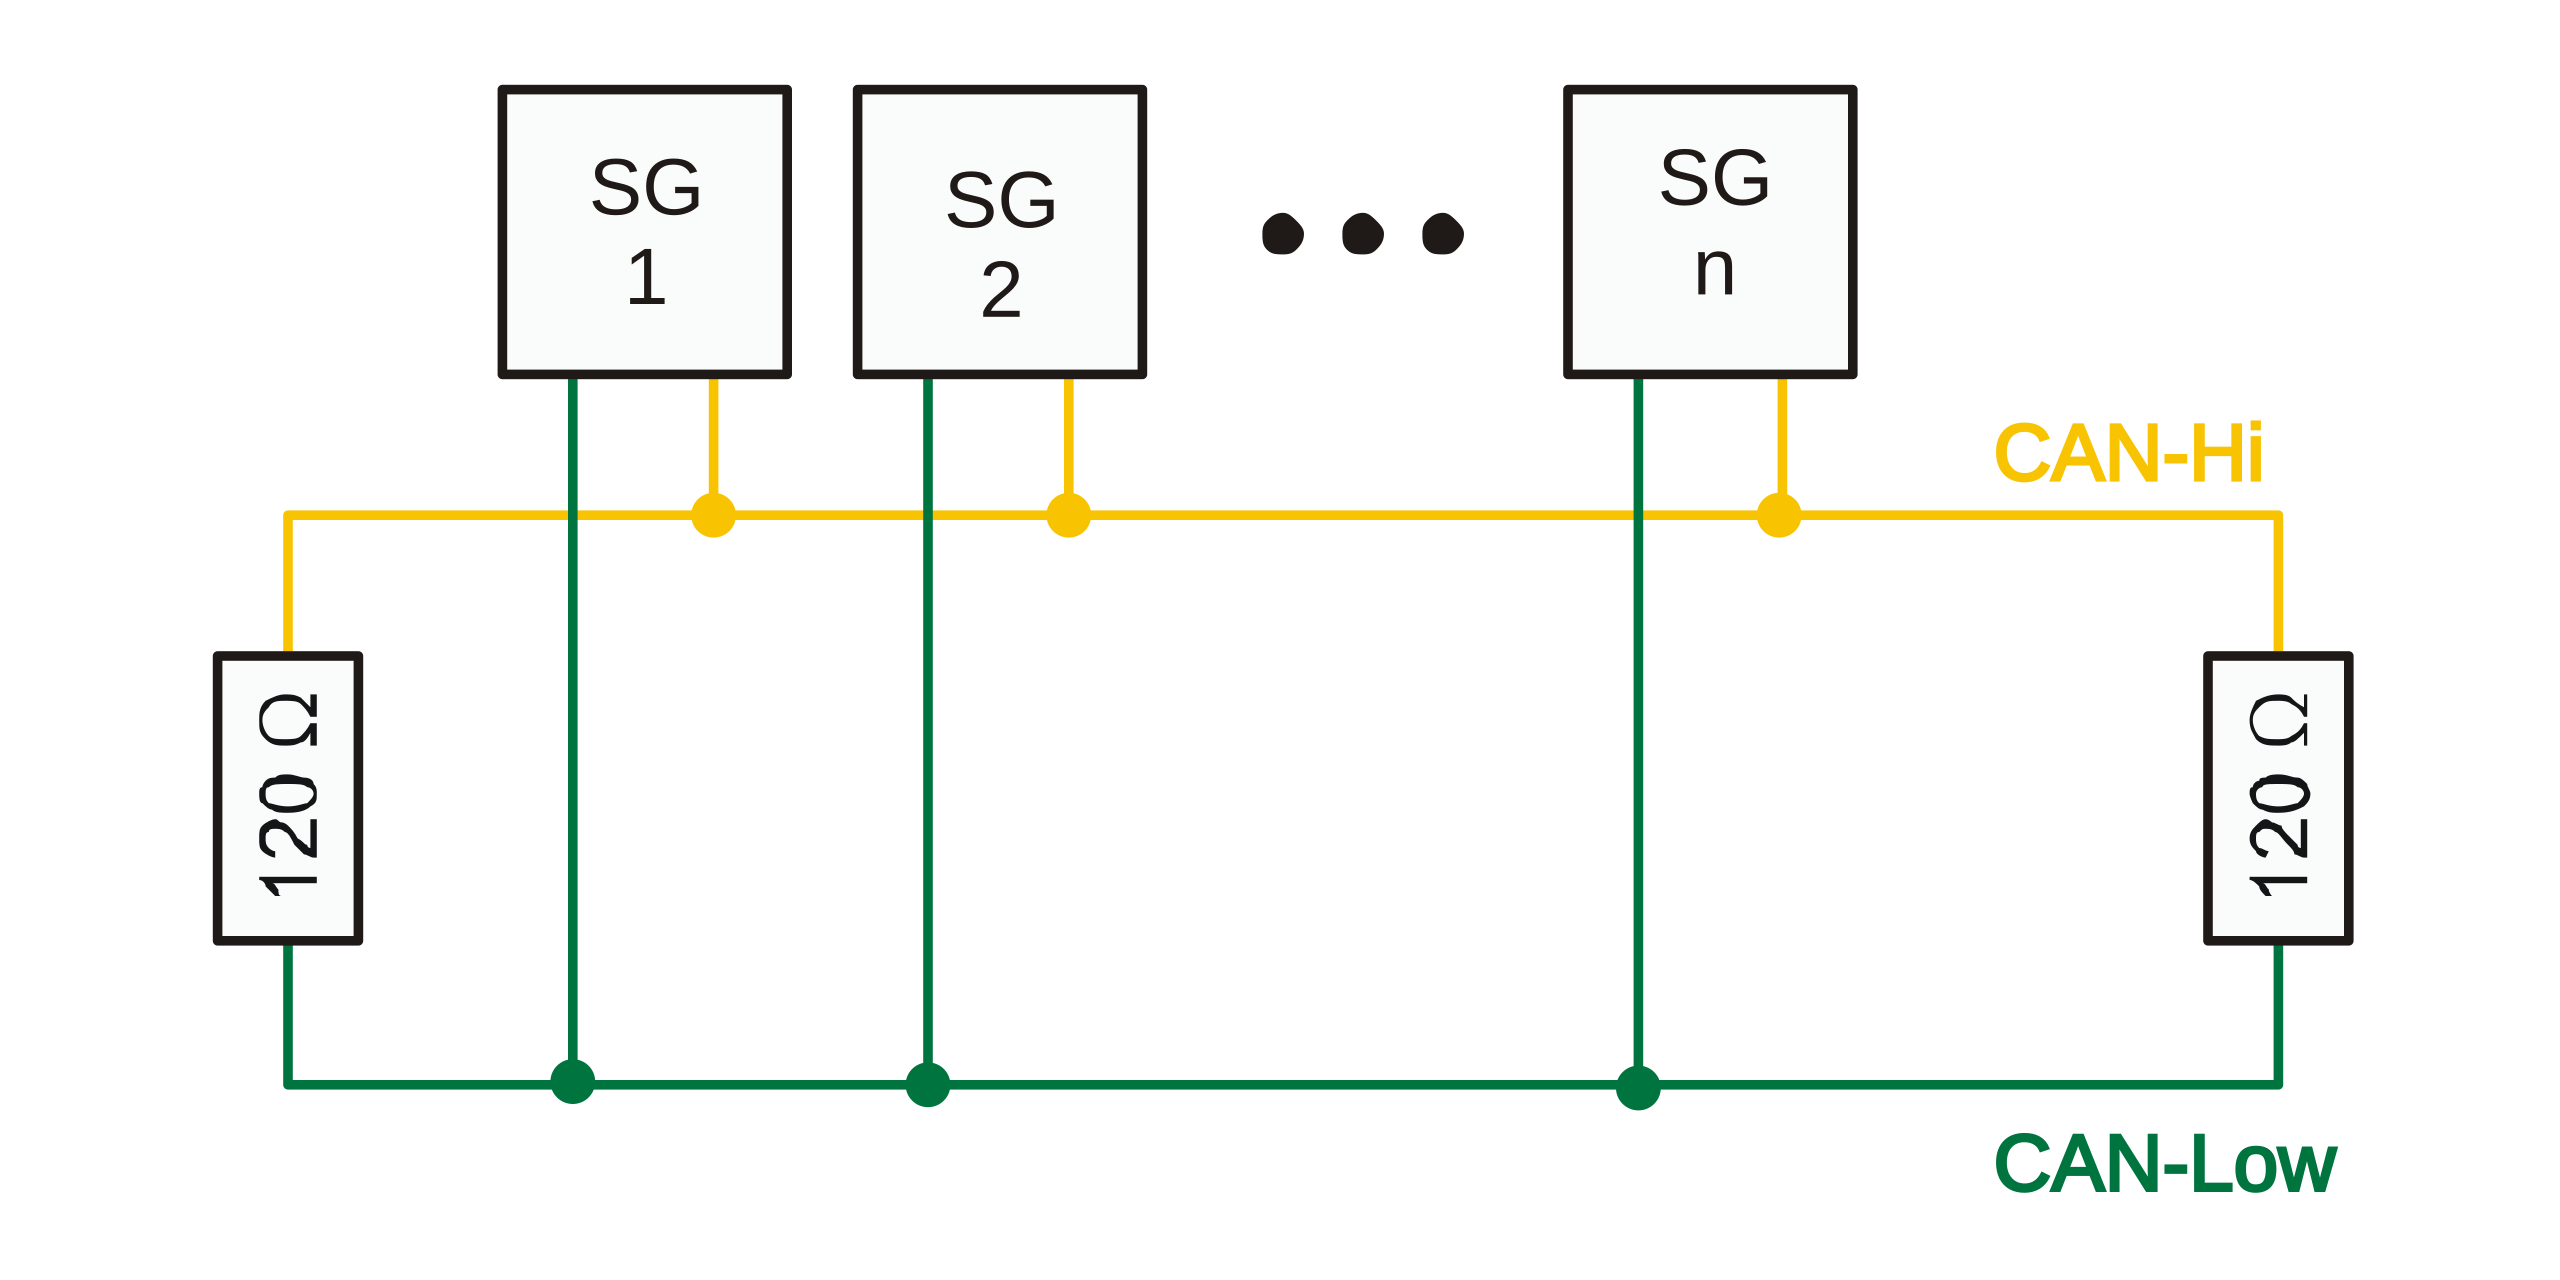
\includegraphics[width=0.4\textwidth]{images/wikipedia_can_bus_topology.png}
    \caption{CAN Bus Topology, Source: Wikipedia \cite{wikipedia_can_bus_image}}
    \label{fig:bus-topology}
\end{figure}

\subsection{Message Structure}
A CAN message consists of a variety of fields, of which the most important are:
\begin{itemize}
    \item \textbf{Arbitration Field/Message identifier:} This field contains the message identifier, which is used to determine message priority. The lower the value of the identifier, the higher the priority of the message.
    \item \textbf{Control Field:} This field contains information about the message, such as the message length.
    \item \textbf{Data Field:} This field contains the actual data being transmitted. In CAN 2.0, this field can contain up to 8 bytes of data.
    \item \textbf{CRC Field:} This field contains a cyclic redundancy check (CRC) to ensure the message's data integrity.
    \item \textbf{Acknowledgement Field:} This field is used to acknowledge the receipt of a message.
\end{itemize}

\noindent Typically, a microcontroller will have a CAN peripheral that handles the low-level details of the CAN protocol, such as message transmission, reception, error detection, etc. The microcontroller's firmware will interact with the CAN peripheral to send and receive messages, as well as configure key parameters such as the bitrate, message filters (only receive certain message ID's), etc.

\subsubsection{CAN Arbitration}
CAN features a unique, \textit{non-destructive} (without data loss), \textit{bit-wise} arbitration mechanism, based on the message identifier. Due to the open-drain nature of the bus, a dominant bit (0) will always override a recessive bit (1). When two nodes start transmitting a message identifier, they constantly monitor the bus to see if the message identifier bit they are transmitting is the same as the message identifier bit on the bus. If a node sees that the message identifier it is transmitting is different from the message identifier on the bus, it will stop transmitting and wait for the bus to become idle before trying to transmit again. Because of this, the node with the lowest message identifier will always win the arbitration and be able to transmit its message (and thus, lower message ID's have higher priority). This is shown in figure \ref{fig:can-arbitration}.

\begin{figure}[H]
    \centering
    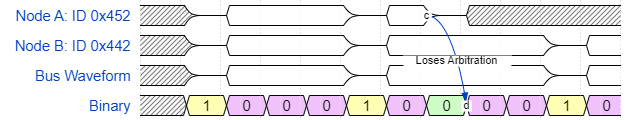
\includegraphics[width=0.8\textwidth]{generated_images/svg_generated/can_bus_arbitration.png}
    \caption{CAN Arbitration Sequence}
    \label{fig:can-arbitration}
\end{figure}

\noindent The CAN arbitration mechanism is one of the key features that make CAN a robust and reliable communication protocol. It ensures that the node with the highest priority message will always be able to transmit its message, even in the presence of multiple nodes trying to transmit messages simultaneously. However, care should be used with low message identifiers, as they can starve (or \textit{step on}) higher message identifiers from transmitting.

\subsection{Follow-ups}
\begin{itemize}
    \item \textbf{Explain how CAN can detect TX errors using TX/RX loopback?}
    \item \textbf{How would you debug a CAN bus that is not working?}
    \item \textbf{What is 'Time Quanta' in CAN?}
\end{itemize}

\end{document}
